% Diagrammes d'architecture avec TikZ pour LaTeX
% À intégrer directement dans le rapport LaTeX

\documentclass[tikz,border=10pt]{standalone}
\usepackage{tikz}
\usetikzlibrary{shapes,arrows,positioning,fit,backgrounds,calc,shadows}

% ============================================
% 1. ARCHITECTURE EN COUCHES
% ============================================
\begin{document}
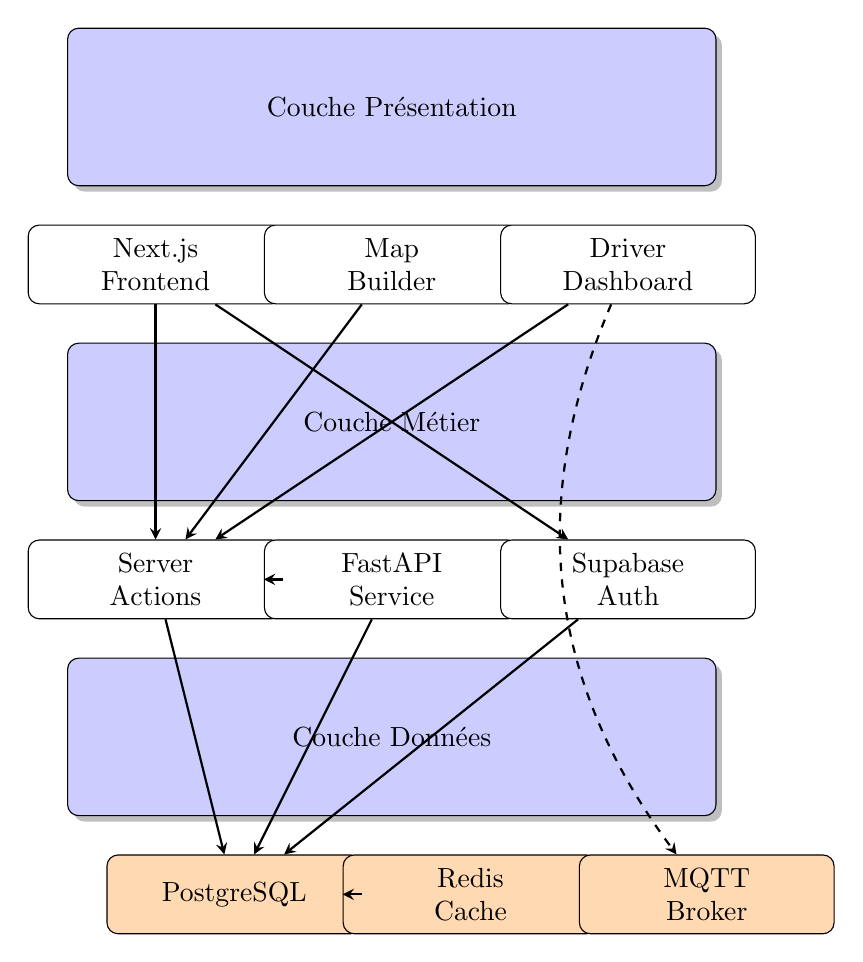
\begin{tikzpicture}[
    layer/.style={rectangle, draw, fill=blue!20, text width=8cm, text centered, rounded corners, minimum height=2cm, drop shadow},
    component/.style={rectangle, draw, fill=white, text width=3cm, text centered, rounded corners, minimum height=1cm},
    arrow/.style={thick,->,>=stealth}
]

    % Couche Présentation
    \node[layer] (pres) at (0,8) {Couche Présentation};
    \node[component] (nextjs) at (-3,6) {Next.js\\Frontend};
    \node[component] (map) at (0,6) {Map\\Builder};
    \node[component] (driver) at (3,6) {Driver\\Dashboard};

    % Couche Métier
    \node[layer] (metier) at (0,4) {Couche Métier};
    \node[component] (sa) at (-3,2) {Server\\Actions};
    \node[component] (fastapi) at (0,2) {FastAPI\\Service};
    \node[component] (auth) at (3,2) {Supabase\\Auth};

    % Couche Données
    \node[layer] (data) at (0,0) {Couche Données};
    \node[component, fill=orange!30] (db) at (-2,-2) {PostgreSQL};
    \node[component, fill=orange!30] (redis) at (1,-2) {Redis\\Cache};
    \node[component, fill=orange!30] (mqtt) at (4,-2) {MQTT\\Broker};

    % Flèches
    \draw[arrow] (nextjs) -- (sa);
    \draw[arrow] (map) -- (sa);
    \draw[arrow] (driver) -- (sa);
    \draw[arrow] (nextjs) -- (auth);

    \draw[arrow] (sa) -- (db);
    \draw[arrow] (sa) -- (fastapi);
    \draw[arrow] (fastapi) -- (db);
    \draw[arrow] (auth) -- (db);

    \draw[arrow] (db) -- (redis);
    \draw[arrow, dashed] (driver) to[bend right=30] (mqtt);

\end{tikzpicture}
\end{document}

% ============================================
% 2. FLUX D'OPTIMISATION (SÉQUENCE)
% ============================================
\begin{document}
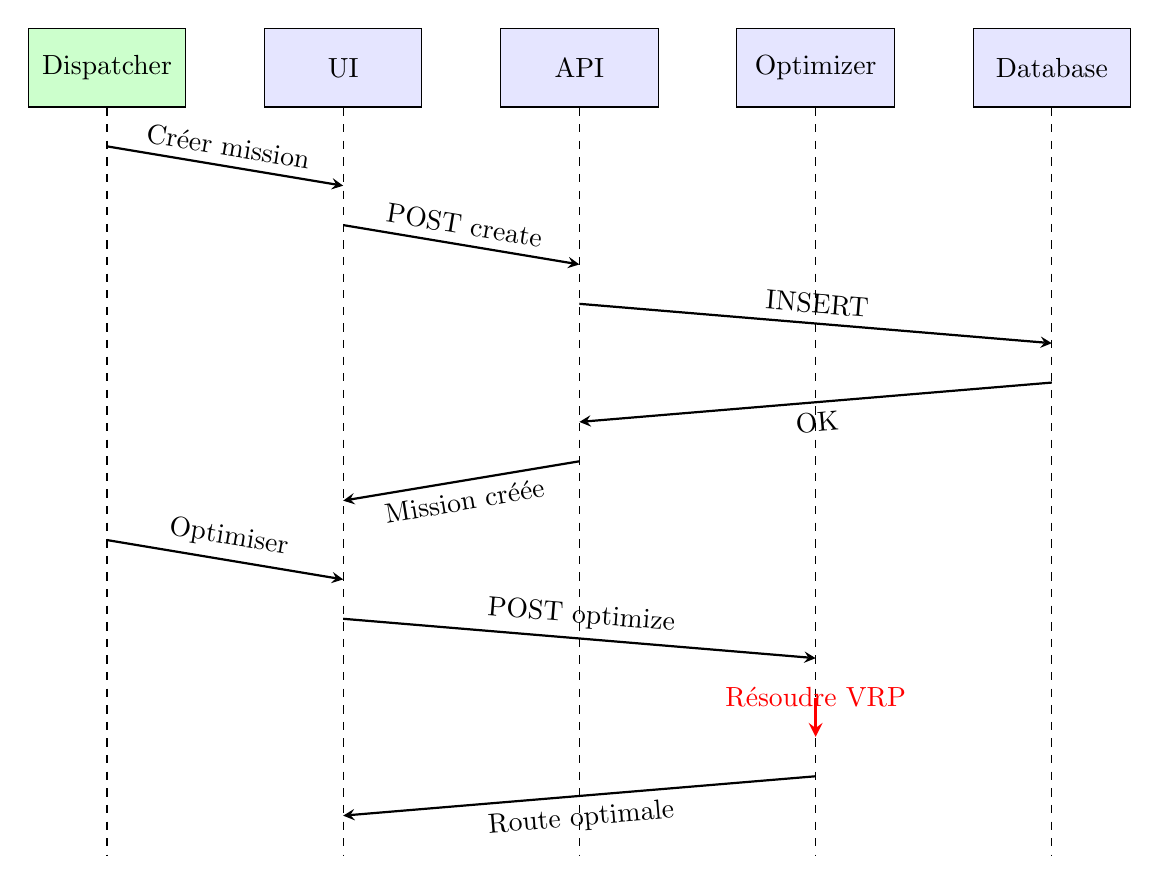
\begin{tikzpicture}[
    actor/.style={rectangle, draw, fill=green!20, minimum width=2cm, minimum height=1cm},
    box/.style={rectangle, draw, fill=blue!10, minimum width=2cm, minimum height=1cm},
    arrow/.style={->,>=stealth, thick}
]

    % Acteurs
    \node[actor] (dispatcher) at (0,0) {Dispatcher};
    \node[box] (ui) at (3,0) {UI};
    \node[box] (api) at (6,0) {API};
    \node[box] (optim) at (9,0) {Optimizer};
    \node[box] (db) at (12,0) {Database};

    % Ligne de vie
    \draw[dashed] (dispatcher) -- (0,-10);
    \draw[dashed] (ui) -- (3,-10);
    \draw[dashed] (api) -- (6,-10);
    \draw[dashed] (optim) -- (9,-10);
    \draw[dashed] (db) -- (12,-10);

    % Messages
    \draw[arrow] (0,-1) -- node[above, sloped] {Créer mission} (3,-1.5);
    \draw[arrow] (3,-2) -- node[above, sloped] {POST create} (6,-2.5);
    \draw[arrow] (6,-3) -- node[above, sloped] {INSERT} (12,-3.5);
    \draw[arrow] (12,-4) -- node[below, sloped] {OK} (6,-4.5);
    \draw[arrow] (6,-5) -- node[below, sloped] {Mission créée} (3,-5.5);

    \draw[arrow] (0,-6) -- node[above, sloped] {Optimiser} (3,-6.5);
    \draw[arrow] (3,-7) -- node[above, sloped] {POST optimize} (9,-7.5);
    \draw[arrow, red, very thick] (9,-8) -- node[above] {Résoudre VRP} (9,-8.5);
    \draw[arrow] (9,-9) -- node[below, sloped] {Route optimale} (3,-9.5);

\end{tikzpicture}
\end{document}

% ============================================
% 3. ARCHITECTURE DE DÉPLOIEMENT
% ============================================
\begin{document}
\begin{tikzpicture}[
    cloud/.style={cloud, draw, fill=blue!10, cloud puffs=10, cloud puff arc=120, aspect=2, minimum width=3cm, minimum height=1.5cm},
    server/.style={rectangle, draw, fill=gray!20, minimum width=2.5cm, minimum height=1.5cm, rounded corners},
    db/.style={cylinder, draw, fill=orange!20, shape border rotate=90, aspect=0.25, minimum height=1.5cm, minimum width=2cm},
    user/.style={circle, draw, fill=green!20, minimum size=1cm}
]

    % Utilisateurs
    \node[user] (users) at (0,6) {Users};

    % CDN
    \node[cloud] (cdn) at (4,6) {CDN\\Cloudflare};

    % Vercel
    \node[cloud, fill=green!10] (vercel) at (8,6) {Vercel\\Next.js};

    % Supabase
    \node[cloud, fill=blue!10] (supabase) at (8,3) {Supabase\\Cloud};
    \node[db] (postgres) at (8,1) {PostgreSQL};

    % AWS
    \node[cloud, fill=orange!10] (aws) at (12,4) {AWS\\Server};
    \node[server] (fastapi) at (12,2) {FastAPI};
    \node[server] (mqtt) at (12,0) {MQTT};

    % Connexions
    \draw[->, thick] (users) -- node[above] {HTTPS} (cdn);
    \draw[->, thick] (cdn) -- (vercel);
    \draw[->, thick] (vercel) -- (supabase);
    \draw[->, thick] (supabase) -- (postgres);
    \draw[->, thick] (vercel) -- (fastapi);
    \draw[->, thick, dashed] (users) to[bend right=20] node[below] {GPS} (mqtt);

\end{tikzpicture}
\end{document}

% ============================================
% 4. MODÈLE DE DONNÉES SIMPLIFIÉ
% ============================================
\begin{document}
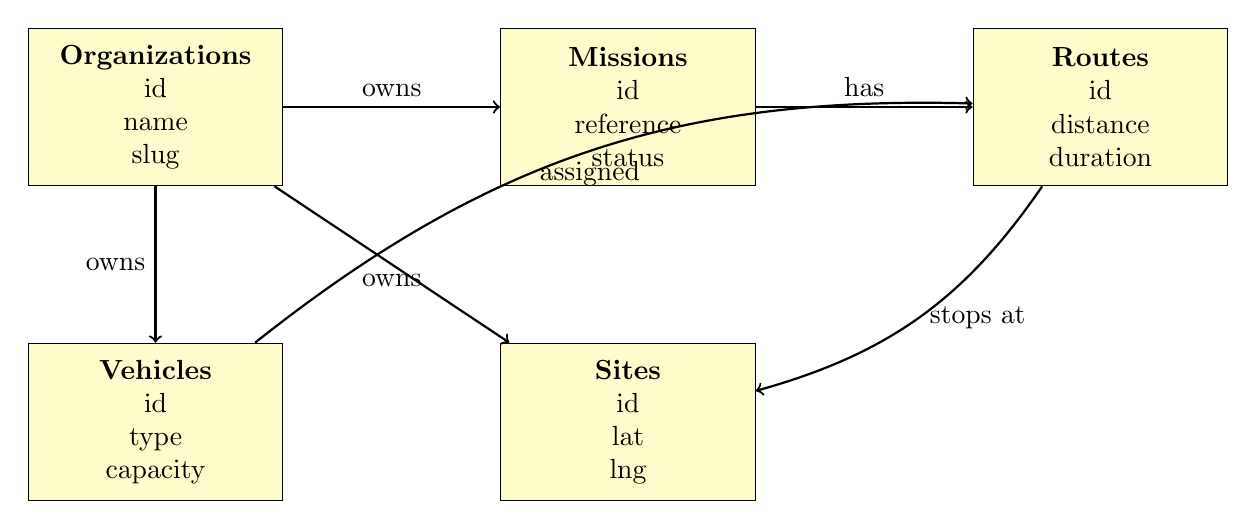
\begin{tikzpicture}[
    entity/.style={rectangle, draw, fill=yellow!20, text width=3cm, align=center, minimum height=2cm},
    relationship/.style={diamond, draw, fill=blue!10, aspect=2},
    attribute/.style={ellipse, draw, fill=green!10}
]

    % Entités principales
    \node[entity] (org) at (0,0) {\textbf{Organizations}\\id\\name\\slug};
    \node[entity] (mission) at (6,0) {\textbf{Missions}\\id\\reference\\status};
    \node[entity] (vehicle) at (0,-4) {\textbf{Vehicles}\\id\\type\\capacity};
    \node[entity] (site) at (6,-4) {\textbf{Sites}\\id\\lat\\lng};
    \node[entity] (route) at (12,0) {\textbf{Routes}\\id\\distance\\duration};

    % Relations
    \draw[->, thick] (org) -- node[above] {owns} (mission);
    \draw[->, thick] (org) -- node[left] {owns} (vehicle);
    \draw[->, thick] (org) -- node[below] {owns} (site);
    \draw[->, thick] (mission) -- node[above] {has} (route);
    \draw[->, thick] (vehicle) to[bend left=20] node[below] {assigned} (route);
    \draw[->, thick] (route) to[bend left=20] node[right] {stops at} (site);

\end{tikzpicture}
\end{document}

% ============================================
% 5. ARCHITECTURE DE SÉCURITÉ (COUCHES)
% ============================================
\begin{document}
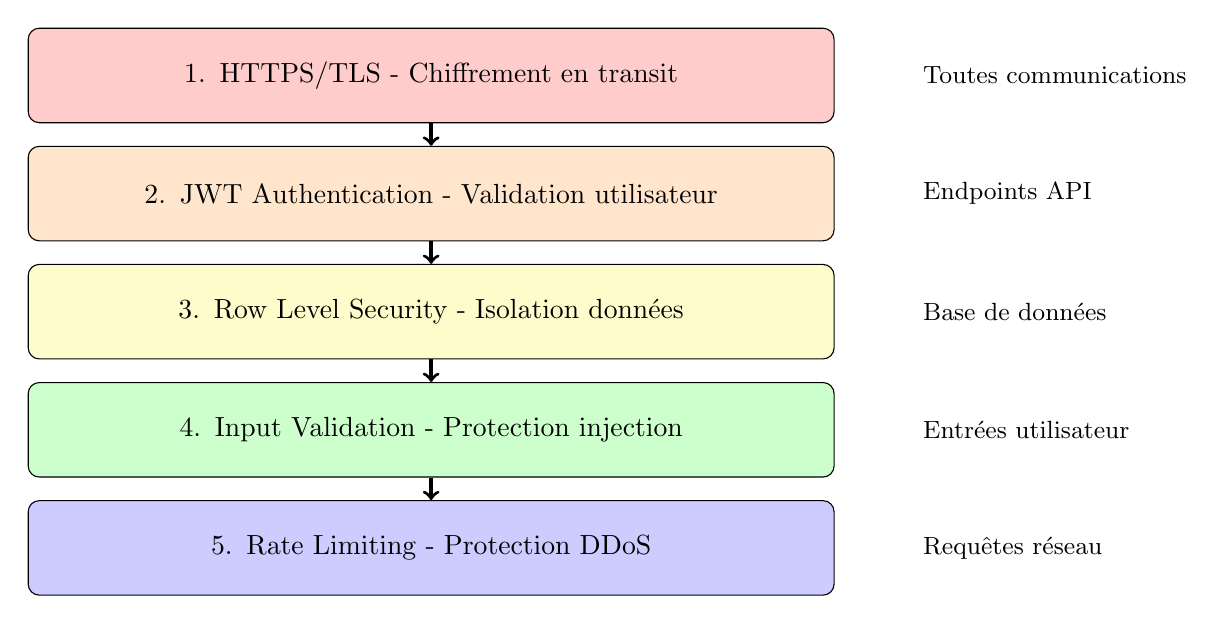
\begin{tikzpicture}[
    security/.style={rectangle, draw, text width=10cm, align=center, minimum height=1.2cm, rounded corners}
]

    \node[security, fill=red!20] (l1) at (0,6) {1. HTTPS/TLS - Chiffrement en transit};
    \node[security, fill=orange!20] (l2) at (0,4.5) {2. JWT Authentication - Validation utilisateur};
    \node[security, fill=yellow!20] (l3) at (0,3) {3. Row Level Security - Isolation données};
    \node[security, fill=green!20] (l4) at (0,1.5) {4. Input Validation - Protection injection};
    \node[security, fill=blue!20] (l5) at (0,0) {5. Rate Limiting - Protection DDoS};

    % Flèches
    \draw[->, very thick] (l1) -- (l2);
    \draw[->, very thick] (l2) -- (l3);
    \draw[->, very thick] (l3) -- (l4);
    \draw[->, very thick] (l4) -- (l5);

    % Labels
    \node[right=1cm of l1] {\small Toutes communications};
    \node[right=1cm of l2] {\small Endpoints API};
    \node[right=1cm of l3] {\small Base de données};
    \node[right=1cm of l4] {\small Entrées utilisateur};
    \node[right=1cm of l5] {\small Requêtes réseau};

\end{tikzpicture}
\end{document}

% ============================================
% 6. PIPELINE CI/CD
% ============================================
\begin{document}
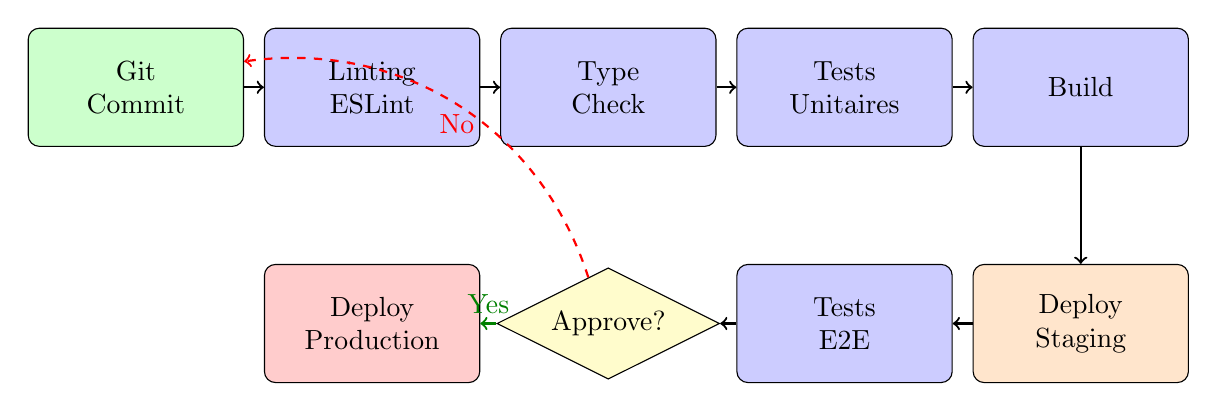
\begin{tikzpicture}[
    stage/.style={rectangle, draw, fill=blue!20, text width=2.5cm, align=center, rounded corners, minimum height=1.5cm},
    decision/.style={diamond, draw, fill=yellow!20, aspect=2, text width=1.5cm, align=center}
]

    % Stages
    \node[stage, fill=green!20] (commit) at (0,0) {Git\\Commit};
    \node[stage] (lint) at (3,0) {Linting\\ESLint};
    \node[stage] (type) at (6,0) {Type\\Check};
    \node[stage] (test) at (9,0) {Tests\\Unitaires};
    \node[stage] (build) at (12,0) {Build};

    \node[stage, fill=orange!20] (staging) at (12,-3) {Deploy\\Staging};
    \node[stage] (e2e) at (9,-3) {Tests\\E2E};
    \node[decision] (approve) at (6,-3) {Approve?};

    \node[stage, fill=red!20] (prod) at (3,-3) {Deploy\\Production};

    % Flèches
    \draw[->, thick] (commit) -- (lint);
    \draw[->, thick] (lint) -- (type);
    \draw[->, thick] (type) -- (test);
    \draw[->, thick] (test) -- (build);
    \draw[->, thick] (build) -- (staging);
    \draw[->, thick] (staging) -- (e2e);
    \draw[->, thick] (e2e) -- (approve);
    \draw[->, thick, green!50!black] (approve) -- node[above] {Yes} (prod);
    \draw[->, thick, red, dashed] (approve) to[bend right=40] node[below] {No} (commit);

\end{tikzpicture}
\end{document}

% ============================================
% INSTRUCTIONS D'UTILISATION
% ============================================
%
% Pour intégrer dans votre rapport LaTeX principal :
%
% 1. Copiez le préambule (packages) dans votre main.tex
% 2. Copiez le code TikZ souhaité dans une figure
%
% Exemple :
%
% \begin{figure}[H]
%     \centering
%     % [Coller le code TikZ ici]
%     \caption{Architecture en couches du système}
%     \label{fig:architecture-couches}
% \end{figure}
%
% Packages requis dans le préambule :
% \usepackage{tikz}
% \usetikzlibrary{shapes,arrows,positioning,fit,backgrounds,calc,shadows}
% \usetikzlibrary{shapes.geometric} % pour cloud
%
